\documentclass[titlepage,a4paper]{jsarticle}
\usepackage{../../sty/import}% 各種パッケージインポート
\usepackage{../../sty/title}% タイトルページの変更
\usepackage{otf}% ローマ数字を使えるようにするやつ
% \usepackage{svg}% SVG画像を読み込めるようにするやつ %なんかコンパイルでなんかしなきゃらしい.面倒そう
\renewcommand{\thesection}{課題\arabic{section}}
%% タイトルページの変数
% レポートタイトル
\title{マーケティング\ajRoman{2}課題まとめ}
% 提出日
\expdate{\today}
% 科目名
\subject{マーケティング\ajRoman{2}}
% 分野
\class{情報経営システム工学分野}
% 学年
\grade{B3}
% 学籍番号
\mynumber{24336488}
% 記述者
\author{本間三暉}
% グループ名 % もし班があるやつならtitle_team.styを入れる
% \team{10}
% 共同実験者 % もし共同実験者が必要なやつならtitle_kyoudou.styを入れる
% \coauthor{%
% \textbf{学籍番号:} & \textbf{氏名:} \\
% \textbf{学籍番号:} & \textbf{氏名:}\\
% \textbf{学籍番号:} & \textbf{氏名:}\\
% \textbf{学籍番号:} & \textbf{氏名:}\\
% }
%
% 記載例:
%\coauthor{%
% 学籍番号:24567321 & 氏名:吉田 富美男 \
% 学籍番号:12345678 & 氏名:安藤 雅洋 \
% 学籍番号:13579234 & 氏名:雲居 玄道 \
%%

\begin{document}
% titleページ作成
\maketitle
\section{スイッチングコストが高いと考える商品、またはサービスをひとつ選び、その概要について説明してください。}
\textbf{選択した商品・サービス:}ERPシステム(企業向けの統合基幹業務システム)

スイッチングコストとは,企業があるITシステムから別のシステムに移行する際に発生するコストや障害のことである.
特にERP(Enterprise Resource Planning)システムは企業の運営に深く関与しているため,その切り替えには時間と費用がかかる.

ERP(Enterprise Resource Planning)システムは,企業が経営資源を一元管理し業務の効率化を図るための統合システムである.
財務管理,人事管理,販売管理,生産管理などの機能が統合されており,企業全体で情報を共有し業務の最適化が可能となる.

ERPシステムのスイッチングコストは非常に高いとされる.
まず,金銭的コストとしては新システムのライセンス費用やハードウェアの追加導入費が発生する.
さらに,既存システムの廃棄に伴う損失も無視できない.
次に,物理的コストとしてデータ移行やシステム統合に要する時間と労力がかかる.
この過程ではデータのバックアップやシステム設定の変更が必要となるため作業負担は大きい.
心理的コストも高く,新システムの操作習得には時間と教育が求められ,従業員の抵抗感も発生し得る.
また,新しいシステムを見つけるまでに要する調査や評価にかかる探索コストも重要である\cite{slide1}.

ERPシステムは,その利便性と引き換えに高いスイッチングコストを伴うため,企業は慎重に検討し導入後の安定運用を確保することが求められる.
スイッチングコストの存在が,企業にとって大きな障壁となることは否めない\cite{slide1}.

\section{独自のポジションを獲得できていると考える商品、または企業をひとつ選び、その特徴を示すポジショニングマップを作成するときの分析軸(2軸)を選び、対象の商品(企業)の位置づけなどについて説明する。}
% ポジショニングマップを示す.%%%
\textbf{選定企業:}アサヒビール(アサヒスーパードライ)
アサヒビールは「アサヒスーパードライ」を発売して以来,「辛口ドライビール」の市場において独自のポジションを確立している\cite{slide1}.
この製品は競合のビール会社との差別化を図りつつ市場で高い認知度を獲得している.

\subsection{分析軸}
\subsubsection{味の特徴(辛口・甘口)}
ドライビールは一般的に「辛口」とされ,キレのある飲み口が特徴である.
アサヒスーパードライは,まさにこの「辛口」を打ち出し,消費者に強い印象を与え続けている.

\subsubsection{価格(高価格・低価格)}
ビール市場においては価格も消費者の選択に大きな影響を与える.
アサヒスーパードライはプレミアムビールほど高価格ではないが,手頃な価格で提供されており大衆的な人気を保ちつつある.

\subsection{ポジショニングマップ}
この2軸でポジショニングマップを作成すると,味の特徴が「辛口」に位置し,価格が「中程度」の位置にアサヒスーパードライを置くことができる.
競合製品としてはキリンやサッポロの類似ドライビールが近い位置に存在するが,
アサヒの「元祖ドライビール」という強いブランド力が独自のポジションを保つ要因となっている.

また,比較対象としてキリン一番,サッポロ黒ラベル,ヱビスビールを挙げる.
味の特徴と価格の2軸を取ってアサヒスーパードライ,キリン一番,サッポロ黒ラベル,ヱビスビールを配置したポジショニングマップを図\ref{map}に示す.
\begin{figure}[H]
  \centering
  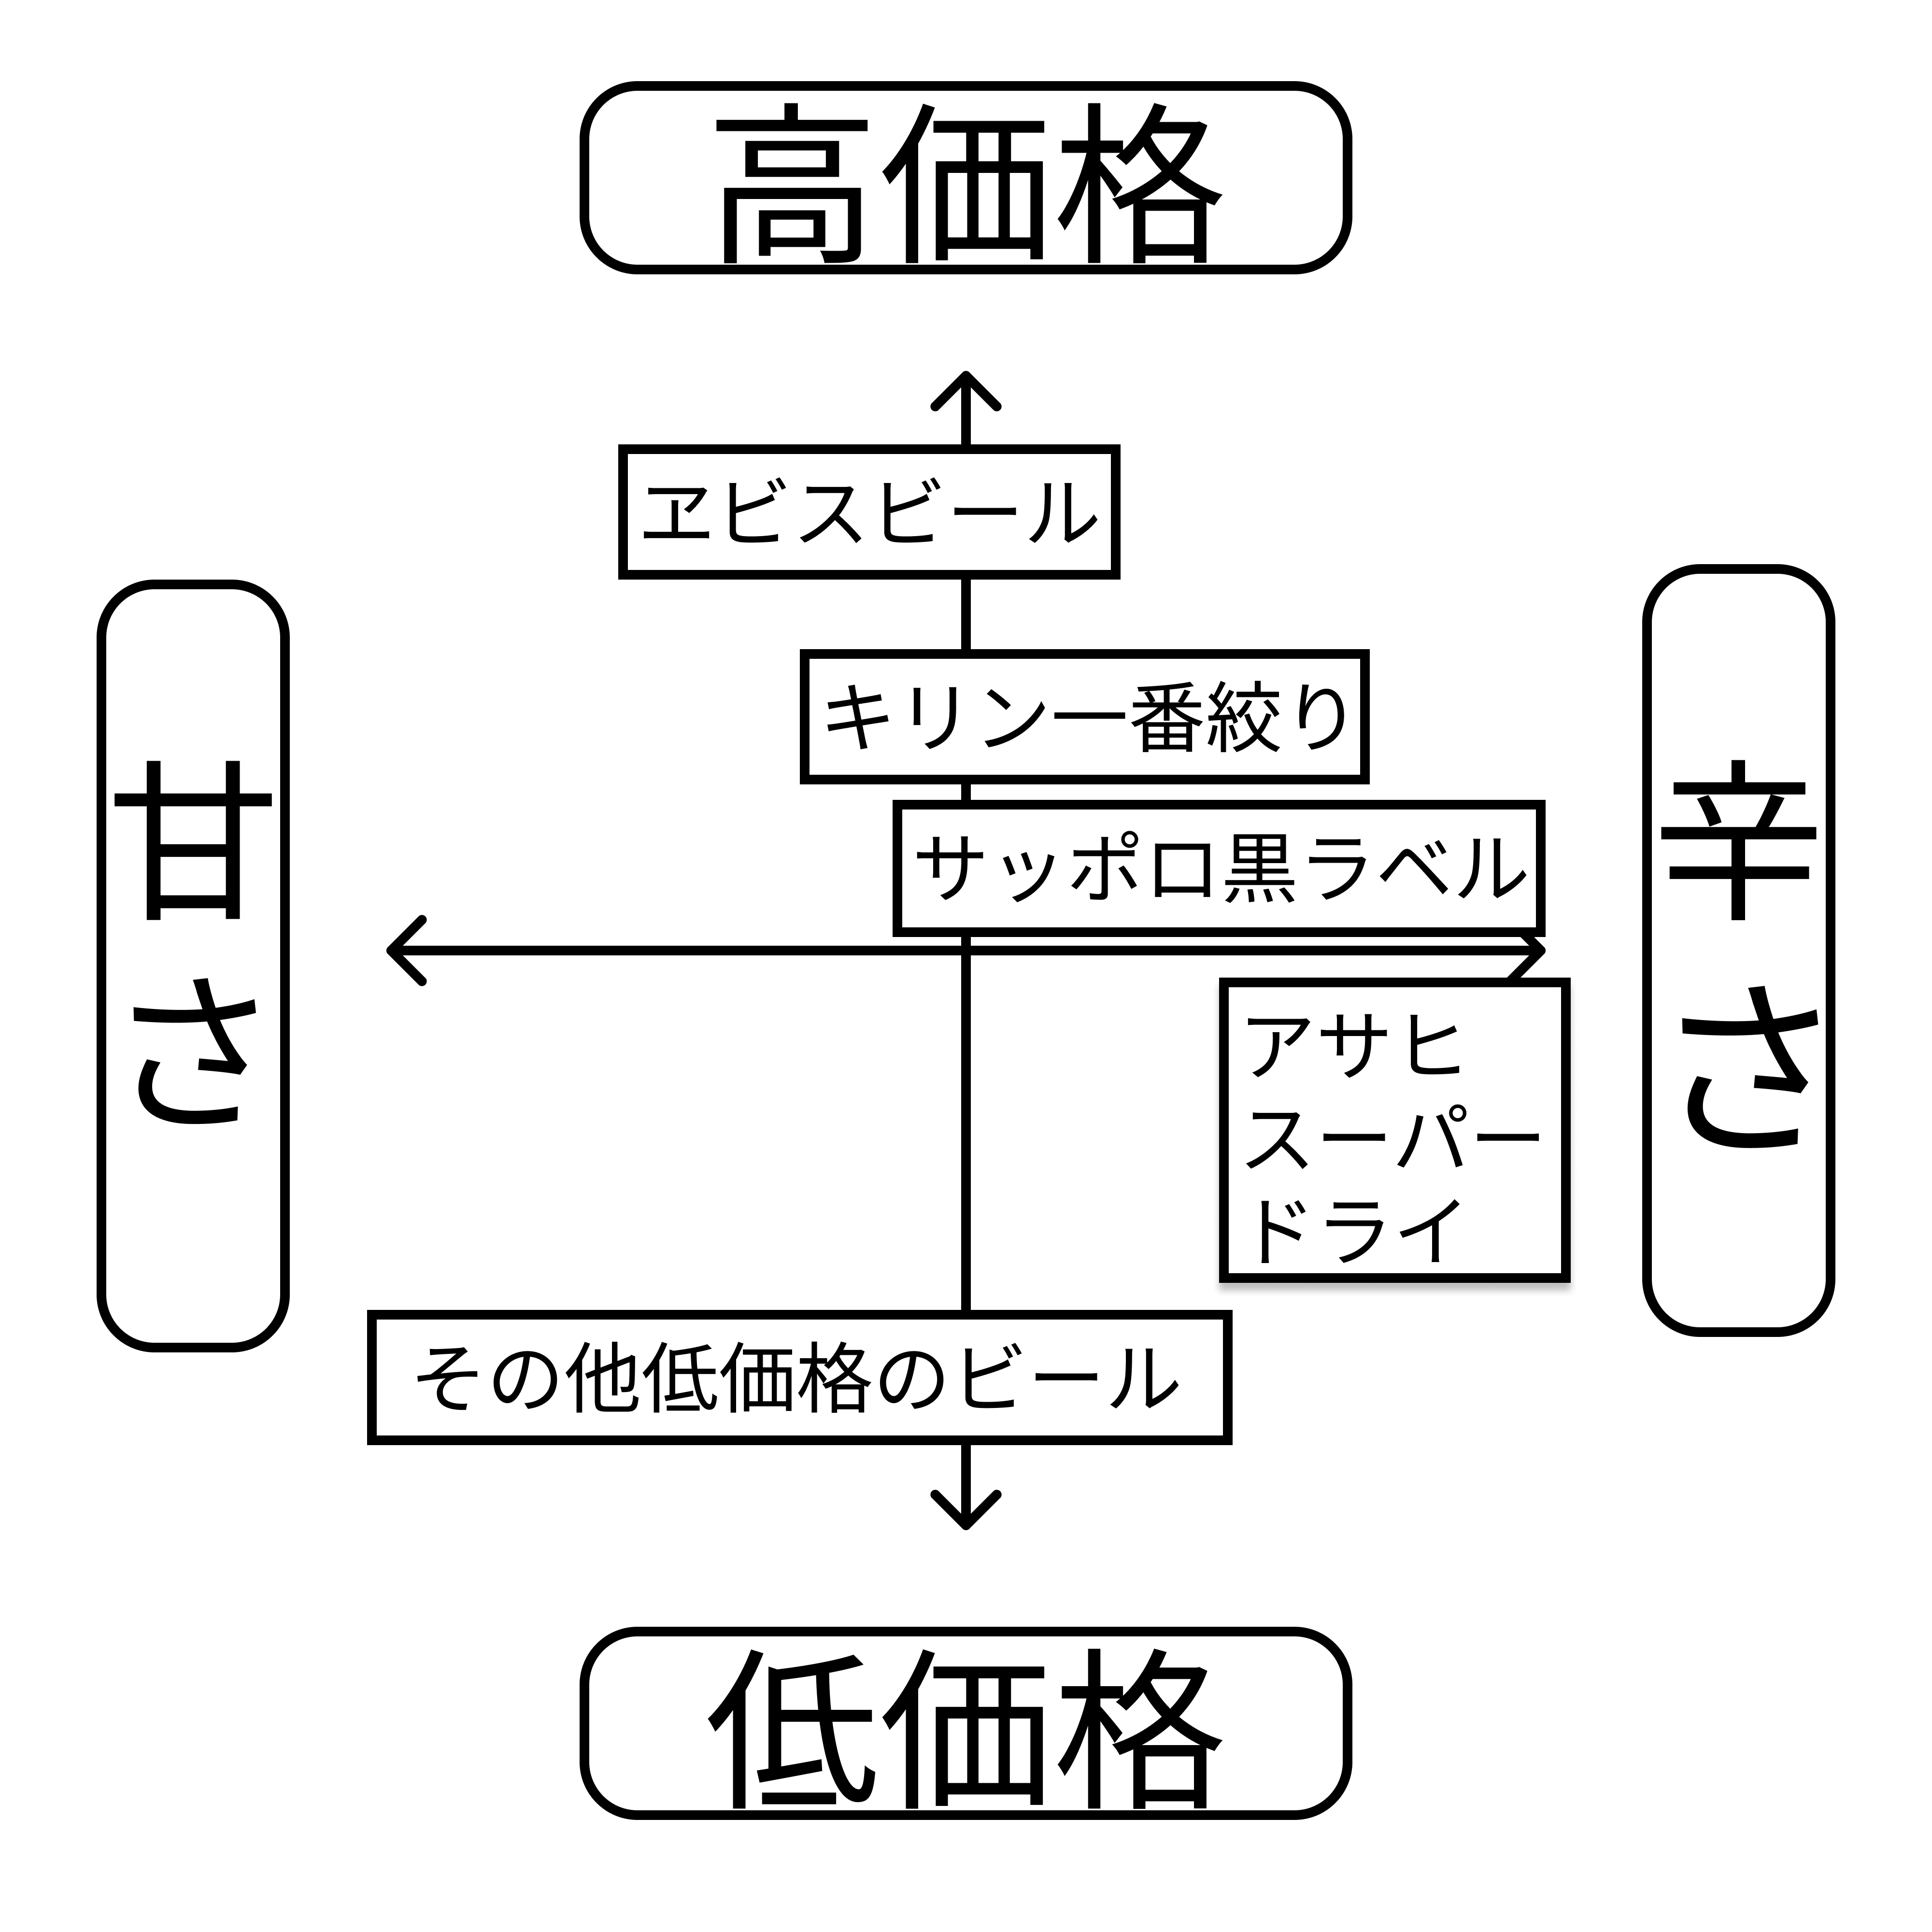
\includegraphics[width=0.8\textwidth]{img/pMap2.png}
  \caption{ビールに関するポジショニングマップ}
  \label{map}
\end{figure}

\subsubsection{キリンビール(キリン一番搾り)}
キリンビールは,その「一番搾り製法」を前面に押し出し,高品質なビールとしてのイメージを確立している.
キリン一番搾りは,麦汁の一番搾り部分だけを使用しており,これによって他のビールとは異なるクリアでスムーズな味わいを提供している.
この製法により,「プレミアム感」や「品質の高さ」を強調し,他社との差別化を図っている.
\\\textbf{軸1:味の特徴(辛口・甘口)}

キリン一番搾りは,アサヒスーパードライに比べてやや「甘口」であり,飲みやすさを強調している.
\\\textbf{軸2:価格(高価格・低価格)}

価格はアサヒスーパードライと同等かやや上の「中価格帯」に位置しているが,「プレミアム感」を打ち出す点で区別されている.

\subsubsection{サッポロビール(サッポロ黒ラベル)}
サッポロビールは,「サッポロ黒ラベル」を代表とする製品で,「男性的で力強いビール」というブランディングを行っている.
サッポロ黒ラベルは長年にわたり「大人のビール」としてのイメージを強く訴求しており,特に成熟した消費者層にアピールしている.
広告キャンペーンでもシンプルさと力強さを前面に出し,他のビールとは一線を画している.
\\\textbf{軸1:味の特徴(辛口・甘口)}

サッポロ黒ラベルは,「中辛口」で,バランスの取れた味わいを提供している.
アサヒスーパードライほどキレが強くはないが,キリン一番搾りよりは辛口である.
\\\textbf{軸2:価格(高価格・低価格)}

サッポロ黒ラベルはアサヒスーパードライやキリン一番搾りと同様に「中価格帯」に位置しており,大衆向けながらも品質を重視したビールである.

\subsubsection{サッポロビール(ヱビスビール)}
エビスビールは,サッポロビールのプレミアムブランドとして,高級感を前面に押し出している.
特に素材や製法にこだわったビールとして,「贅沢さ」や「上質さ」を強調しプレミアムビール市場において確固たる地位を築いている.
\\\textbf{軸1:味の特徴(辛口・甘口)}

ヱビスビールは「やや甘口」で,リッチでまろやかな味わいを提供する.
\\\textbf{軸2:価格(高価格・低価格)}

ヱビスビールは「高価格帯」に位置し,特に特別なシーンや贈答用として消費者に選ばれている.

\section{日本にあるコンビニで販売されている弁当の年間売上高を推計してください。}
コンビニ弁当の年間売上高を推計するには,大手3社(セブンイレブン,ローソン,ファミリーマート)のデータをもとに考える必要がある.
まず市場規模を導出するための計算式を式\eqref{con},\eqref{jpn}に示す.
\begin{align}
  \text{コンビニの弁当売上} =& \text{コンビニの売上高} \times \text{日配食品(弁当などの短期消費品)の割合}\label{con}\\
  \text{日本の弁当の年間売上高} =& \text{コンビニ大手3社の弁当売上} \times \frac{\text{日本のコンビニの総店舗数}}{\text{大手3社の総店舗数}}\label{jpn}
\end{align}
以下の小節で詳しい計算を行う.
 
\subsection{セブンイレブン}
セブンイレブンは2023年に約5.1兆円の売上高を記録しており,そのうち日配食品(弁当などの短期消費品)の割合は約12.5\%である\cite{711}.
この割合をもとに,弁当などの売上は約6375億円と推定される.

\subsection{ローソン}
ローソンの全体の売上高は約2.5兆円で,同じく日配食品の売上が占める割合が大きい.
仮に同様に12.5\%と仮定すると,ローソンにおける弁当などの売上は約3125億円と推定できる\cite{Lowson}.

\subsection{ファミリーマート}
ファミリーマートは売上高が約3兆円で,こちらも同様に日配食品が12.5\%と仮定すれば,弁当売上は約3750億円となる\cite{fam}.

\subsection{その他コンビニの売上}
各コンビニの売上割合がほぼ等しいものとした時,コンビニ業大手3社とその他のコンビニの店舗数を比べることでまとめて比較することができると考えた.
2023年度の大手3社の総店舗数はおよそ5万店舗ほど,その他コンビニの総店舗数はおよそ5000店舗である\cite{conven}.
そのため,同じような売上をあげれると考えると,日本のコンビニ全体での弁当の年間売上は大手3社の弁当の年間売上の1.1倍程度であると考える.

\subsection{推定結果}
以上を総合すると,セブンイレブン,ローソン,ファミリーマートの弁当の年間売上高は,合計で約1.32兆円と推定される.
これに他の小規模コンビニチェーンの売上が加わることを考えると,日本のコンビニ全体での弁当の年間売上はおよそ1.45兆円程度になると考えられる.

\section{企業(業種などは任意)のマーケティングにとって有効なデータを選び、IoTデバイスを用いたデータの収集方法を検討し、説明する。}
企業のマーケティングにおいて有効なデータとして\textbf{消費者行動データ}を選定する.
消費者行動データは購買傾向や来店頻度,興味・関心の商品カテゴリを把握するのに有効である.
このデータを用いることで,マーケティング戦略の最適化が可能となりプロモーションの効果を最大化するためのターゲティング精度が向上する.

\subsection*{IoTデバイスを用いたデータ収集方法:}%%%
% \subsection{スマートフォン連携センサー}
% IoTデバイスとして店舗内に配置されたセンサーが,スマートフォンと連携することで来店客の行動データを収集できる.
% 例えば,Wi-FiやBluetoothを利用して顧客がどの棚に長く滞在していたか,どの商品の前で足を止めたかを把握する.
% この情報を基に,店内レイアウトの最適化やプロモーション展開のタイミングを調整できる.

% \subsection{スマートシェルフ}
% スマートシェルフは商品の在庫や売れ行きのデータをリアルタイムで記録し,消費者がどの商品を手に取ったか,または戻したかなどの詳細なデータを収集できる.
% これにより,特定商品の売上状況だけでなく消費者の関心度を高める商品の配置方法を改善できる.

% 具体的な方法としては
% \subsection{ウェアラブルデバイス}
% 特定の業種では顧客にウェアラブルデバイスを提供し,心拍数や移動パターンを分析することで商品の購買意欲を高める環境づくりに役立てることができる.
% 例えば,フィットネスクラブなどでは顧客の運動データを基にした商品やサービスの提案が可能となる.

\subsection{スマートシェルフ}
スマートシェルフは,IoT技術を活用してリアルタイムで商品に関するデータを収集するシステムであり,企業のマーケティングや在庫管理を効率化するための重要なツールである.
以下では,スマートシェルフに絞り込み,その具体的なデータ収集方法と活用について詳述する.

\subsection{データ収集の仕組み}
スマートシェルフは,棚に設置されたセンサーやRFID(無線タグ),カメラなどを用いて,次のようなデータをリアルタイムで収集する.

\subsubsection{在庫状況}
各商品が棚にどれだけ残っているかをリアルタイムで検知する.
RFIDや重量センサーにより,商品の追加や減少が記録され,在庫切れを防ぐために自動でアラートが出される.

\subsubsection{消費者の行動}
顧客が棚から商品を手に取る回数や戻す回数,どの時間帯に商品がよく取られるかといったデータも収集できる.
これにより,特定の商品の注目度や顧客の関心動向を可視化できる. 

\subsubsection{購買データの統合}
スマートシェルフはセブンイレブンを始めとした小売業界や飲食店などで広く使用されているPOSシステムと連携することで,
消費者が実際にどの商品を購入したか,その購買行動との関連を把握することも可能である.
これにより,棚の配置やマーケティングキャンペーンの効果を追跡する.

\subsection{データの活用方法}
収集されたデータは企業のマーケティングや在庫管理において多岐にわたって活用される.
まず,在庫管理の最適化が可能となり商品の在庫レベルをリアルタイムで把握することで,在庫切れや過剰在庫を防ぎ補充スケジュールを自動化することができる.
特に需要の変動が激しい商品に対しては迅速な対応が可能になり,売れ筋商品を特定して売り場スペースを最適化することで販売機会を逃さないようにできる.

また,顧客がどの商品を手に取り,どれを戻したかといった行動データを分析することでマーケティングキャンペーンの効果を測定することもできる.
たとえば,特定の商品の注目度が広告キャンペーン後にどう変わったかを評価し,それに基づいて新たなプロモーションや価格戦略の見直しを行う.

消費者行動のデータをさらに活用し,どの時間帯にどの商品がよく売れるかを分析することで顧客の行動パターンに合わせたパーソナライズされたプロモーションを展開することができる.
特定の時間帯に購買が集中する商品にはタイムセールや特別プロモーションを実施することが効果的である.

さらに,リアルタイムで商品が在庫切れに近づいた際にアラートを発するなどで自動的に補充手配が行われることで,販売機会を逃さず顧客満足度を向上させることができる.

\subsection{具体例と展開の可能性}
イオンやウォルマートといった大手スーパーマーケットチェーンで導入されているスマートシェルフは,店舗運営の効率化に成功しており全店舗での導入が進んでいる.
このようなシステムは,特に消費者のニーズが高まる季節やイベント時に有効であり,需要予測と販売戦略を強化するために欠かせないツールとなっている.
また,スマートシェルフは,BtoBの分野においても,工場や物流センターでの資材管理に利用されるケースも増えている.

\section{ひとつのモノ(商品・サービス)を任意で選び、選定したモノとそれと競合するモノをひとつ以上選んだうえで、それぞれを分類するマトリクスを作成する。
  マトリクスの作成においては、モノの特徴を考慮し、縦軸の上下、横軸の左右、それぞの分析軸を示す。
  選んだモノ、および競合するモノをプロットしたうえで、それぞれの特徴をターゲットとともに説明してください。}%%%
% 課題2と同じ感じのやつ
% 浅野「スマートフォン良くね」
選定するモノとしてiPhoneシリーズを選ぶ.
また,iPhoneシリーズと競合するモノとして他のスマートフォンシリーズである,Galaxy,Pixel,Redmi,OnePlus,Xperiaなどが挙げられる.
\subsection{分析軸}
\subsubsection{性能(高性能・低性能)}
スマートフォンの性能にはプロセッサのスピード,カメラの画質,メモリの容量,バッテリーの持続時間などが関係する.
高性能なスマートフォンはゲーマーやクリエイティブ業務を行うユーザー向けであり,
一方,性能がそこまで求められないユーザーにはコストパフォーマンス重視のモデルが人気である.
\subsubsection{価格(高価格・低価格)}
価格はターゲットに大きく影響を与える要因である.
高価格帯のスマートフォンは最新の技術やデザインを搭載しており,プレミアムなユーザー層(ビジネスパーソンや技術愛好家)に適している.
低価格帯のスマートフォンは,学生や価格に敏感なユーザー向けである.
\subsection{ポジショニングマップ}
それらを分類するために2軸として価格と性能を用いたポジショニングマップを図\ref{smart}に示す.
\begin{figure}[H]
\centering
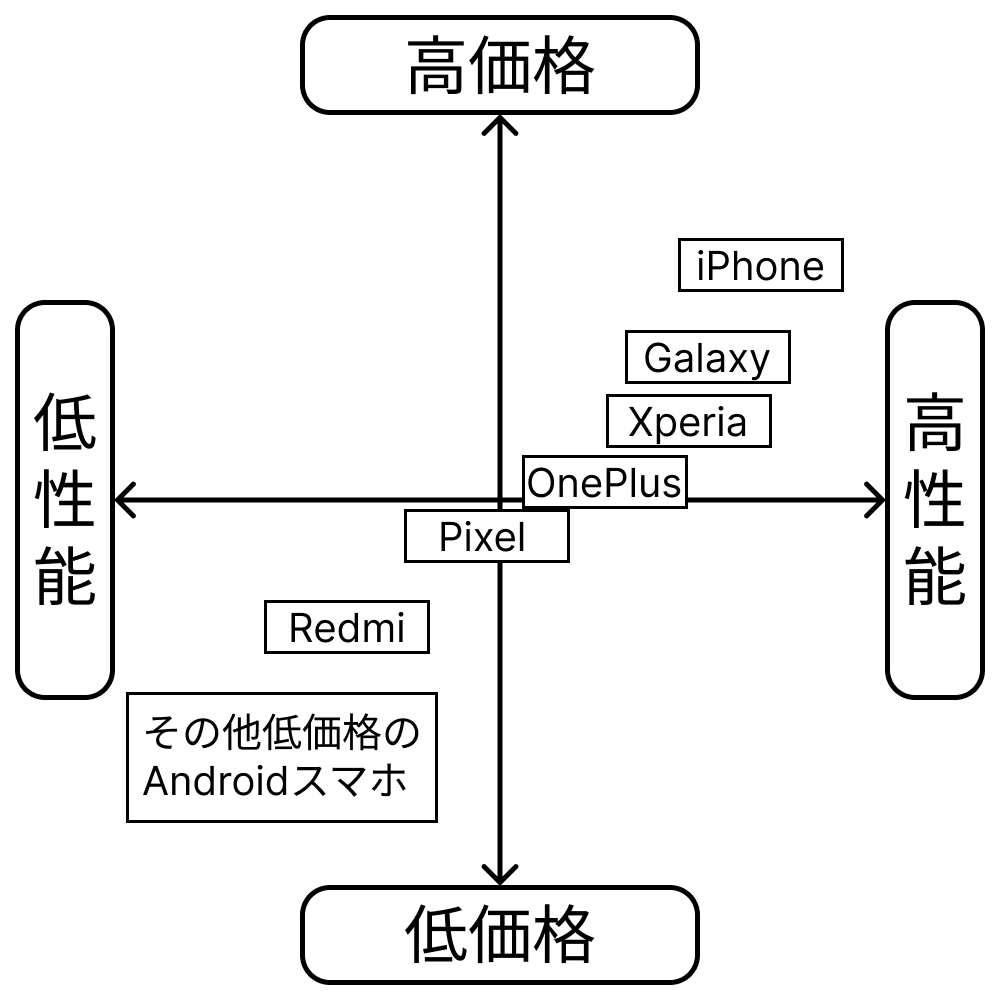
\includegraphics[width=0.8\textwidth]{img/pMap3.png}
\caption{スマートフォンに関するポジショニングマップ}
\label{smart}
\end{figure}

\subsection{Apple iPhoneシリーズ}
\subsubsection{特徴}
Apple製のフラッグシップスマートフォン.
iOSを搭載し,Appleのエコシステムとの強い連携が特徴.優れたデザイン,使いやすさ,
セキュリティ,そして高品質なカメラやディスプレイが評価されている.
\subsubsection{価格}
高価格帯(約10万~15万円)
\subsubsection{性能}
Appleの最新Aシリーズチップを搭載しており,
全体的なパフォーマンスは業界トップクラス.カメラ性能,ディスプレイ品質,そしてバッテリー効率も非常に高い.
\subsection{Samsung Galaxyシリーズ}
\subsubsection{特徴}
Samsungの主力Androidスマートフォン.AMOLEDディスプレイの美しさや,マルチタスクをサポートするSペン(Noteシリーズなど),多機能カメラが強み.
\subsubsection{価格}
中~高価格帯(約8万~15万円)
\subsubsection{性能}
最新のExynosまたはSnapdragonチップを搭載.特にディスプレイとカメラの性能が際立っており,性能面ではiPhoneに次ぐトップクラス.
\subsection{Google Pixelシリーズ}
\subsubsection{特徴}
Google純正のAndroidスマートフォン.Android OSの最新バージョンをいち早く利用でき,GoogleのAI機能(特にカメラ処理)を活用したソフトウェアが強み.
シンプルなUIも特徴.
\subsubsection{価格}
中価格帯(約6万~9万円)
\subsubsection{性能}
Google独自のTensorチップを搭載し,AIベースの機能が充実.
カメラのソフトウェア処理が優れており,特に夜間撮影やポートレート撮影で高い評価を受けている.
ハードウェア性能はiPhoneやGalaxyには劣るが,十分なパフォーマンスを提供.
\subsection{Xiaomi Redmiシリーズ}
\subsubsection{特徴}
特徴: 高性能なスペックを低価格で提供することを特徴とするXiaomiのミドルレンジスマートフォンブランド.
特に新興国や価格に敏感な市場で人気.
\subsubsection{価格}
低価格帯(約2万~5万円)
\subsubsection{性能}
ミドルクラスのプロセッサを搭載し,日常的なタスクやライトなゲームには十分対応可能.
カメラ性能やディスプレイ品質は他のハイエンドモデルには及ばないが,コストパフォーマンスは非常に高い.
\subsection{OnePlusシリーズ}
\subsubsection{特徴}
高性能ながら比較的手頃な価格を提供することを目指したスマートフォン.
クリーンなAndroid体験と高性能スペックが特徴で,特に技術愛好家やゲーマーに人気がある.
\subsubsection{価格}
中価格帯(約5万~9万円)
\subsubsection{性能}
Snapdragonのハイエンドチップを搭載し,ディスプレイや充電速度も優れている.
特にゲーマーやパワーユーザー向けに最適化された機能が多い.
\subsection{Sony Xperiaシリーズ}
\subsubsection{特徴}
高解像度ディスプレイや,特に映像・音楽関連の技術に強みを持つSonyのフラッグシップスマートフォン.
4K OLEDディスプレイやハイレゾ音源対応など,クリエイターや音楽愛好家向けの機能が豊富.
\subsubsection{価格}
中~高価格帯(約7万~13万円)
\subsubsection{性能}
高性能プロセッサを搭載し,特にディスプレイやカメラ性能が強化されている.
動画撮影機能に特化したモデルもあり,クリエイティブ業務に向いたスペック.
% 参考文献
\begin{thebibliography}{99}
  \bibitem{slide1} 令和6年 マーケティング\ajRoman{2}授業スライド
  \bibitem{711} セブンイレブンの公式データ\url{https://www.sej.co.jp/company/yokogao/data/}
  \bibitem{Lowson} ローソンIR資料\url{https://www.lawson.co.jp/company/ir/library/annual_report/2022/pdf/ar2022_P64-67.pdf}
  \bibitem{fam} ファミリーマートの分析記事\url{https://smbiz.asahi.com/article/14601977}
  \bibitem{conven} 【2024年版】コンビニエンスストアの店舗数ランキング|日本ソフト販売株式会社\url{https://www.nipponsoft.co.jp/blog/analysis/chain-conveniencestore2024/}
  \bibitem{IoT} IoTスマートシェルフの概要と活用事例 \url{https://www.iotjournal.com/articles/solution/iot-smart-shelf/}
  \bibitem{shelf} スマートリテールの最新動向\url{https://retailjournal.jp/smart-retail/2023/}
\end{thebibliography}

\end{document}